
\subsection*{Hint for Review  Question~\ref{orthogprob}}

%%%Insert this to get the typewriter font so it looks like a real movie script
{\ttfamily
\fontdimen2\font=0.4em
\fontdimen3\font=0.2em
\fontdimen4\font=0.1em
\fontdimen7\font=0.1em
\hyphenchar\font=`\-


You are asked to consider an orthogonal basis $\{v_1,v_2,\ldots v_n\}$.
Because this is a basis any $v\in V$ can be uniquely expressed as
$$
v=c^1 v_1 + c^2 v_2 +\cdots +v^n c_n\, ,
$$
and the number $n=\dim V$. Since this is an orthogonal basis
$$
v_i\dotprod v_j =0 \, ,\qquad i\neq j\, .
$$
So different vectors in the basis are orthogonal:
\begin{center}
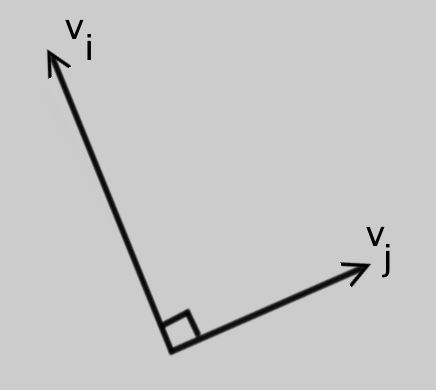
\includegraphics[scale=.4]{\orthonormPath/rightangles.jpg}
\end{center}
However, the basis is {\it not} orthonormal so we know nothing about the
lengths of the basis vectors (save that they cannot vanish). 

To complete the hint, lets use the dot product to compute a formula for $c^1$ in terms of the basis vectors and $v$. Consider
$$
v_1\dotprod v = c^1 v_1\dotprod v_1 + c^2 v_1\dotprod v^2 +\cdots + c^n v_1\dotprod v_n=c^1 v_1\dotprod v_1\, .
$$
Solving for $c^1$ (remembering that $v_1\dotprod v_1\neq 0$) gives
$$
c^1 = \frac{v_1\dotprod v\ }{v_1\dotprod v_1}\, .
$$
This should get you started on this problem.

} % Closing bracket for font

%\newpage
